\documentclass{standalone}
\usepackage{tikz}
\begin{document}
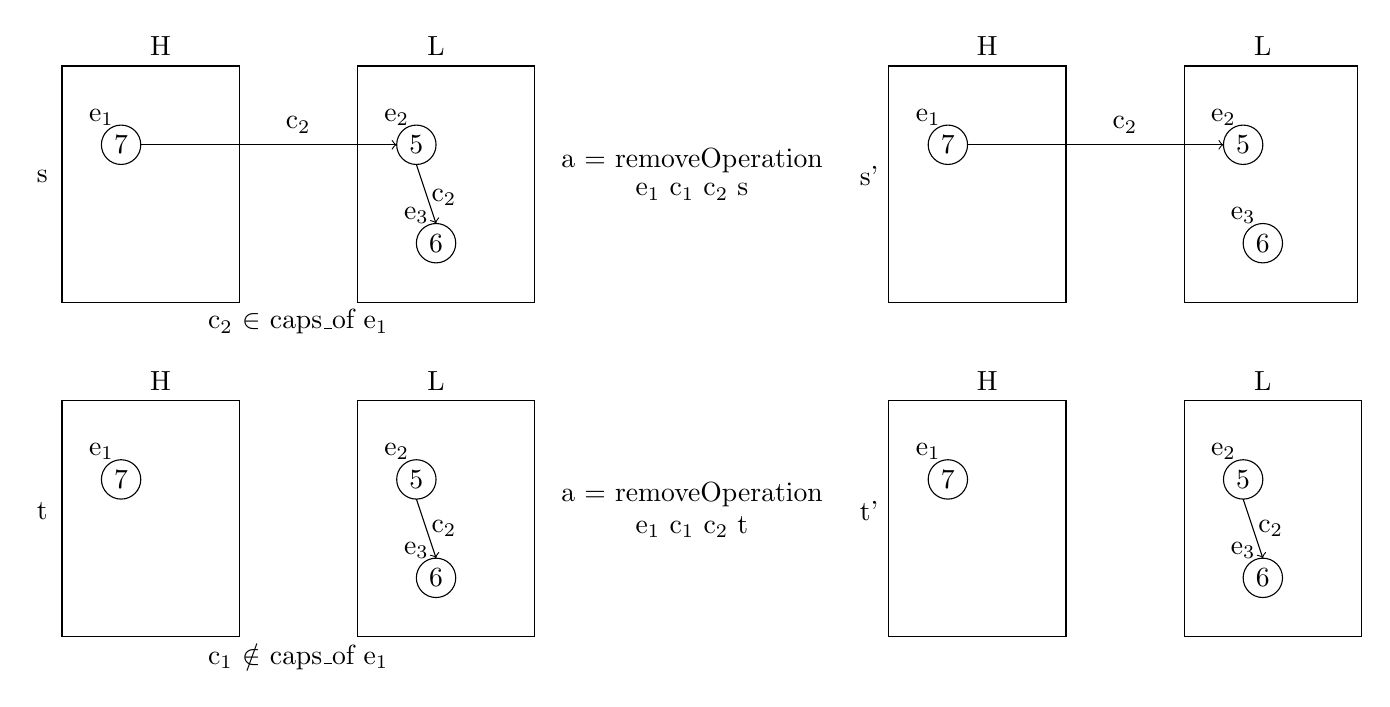
\begin{tikzpicture}
\node at (0,1.6) {t};
\node at (1.5,3.25) {H};
\draw [black] (0.25,0) rectangle (2.5,3);
\draw [black] (4,0) rectangle (6.25,3);
\draw [black] (1,2) circle [radius=0.25] node {7};
\node at (0.75,2.35) {e$_1$};
\node at (5,3.25) {L};
\draw [black] (4.75,2) circle [radius=0.25] node {5};
\node at (4.5,2.35) {e$_2$};
\draw [black] (5,0.75) circle [radius=0.25] node {6};
\node at (4.75,1.1) {e$_3$};
\draw [->, black] (4.75,1.75) -- (5,1);
\node at (5.1,1.375) {c$_2$};
\node at (3.25,-0.25) {c$_1$ $\notin$ caps$\_$of e$_1$};
\node at (8.25,1.8) {a = removeOperation};
\node at (8.25,1.4) {e$_1$ c$_1$ c$_2$ t};
\node at (10.5,1.6) {t'};
\node at (12,3.25) {H};
\draw [black] (10.75,0) rectangle (13,3);
\draw [black] (14.5,0) rectangle (16.75,3);
\draw [black] (11.5,2) circle [radius=0.25] node {7};
\node at (11.25,2.35) {e$_1$};
\node at (15.5,3.25) {L};
\draw [black] (15.25,2) circle [radius=0.25] node {5};
\node at (15,2.35) {e$_2$};
\draw [black] (15.5,0.75) circle [radius=0.25] node {6};
\node at (15.25,1.1) {e$_3$};
\draw [->, black] (15.25,1.75) -- (15.5,1);
\node at (15.6,1.375) {c$_2$};

\node at (0,5.85) {s};
\node at (1.5,7.5) {H};
\draw [black] (0.25,4.25) rectangle (2.5,7.25);
\draw [black] (4,4.25) rectangle (6.25,7.25);
\draw [black] (1,6.25) circle [radius=0.25] node {7};
\node at (0.75,6.6) {e$_1$};
\node at (5,7.5) {L};
\draw [->, black] (1.25,6.25) -- (4.5,6.25);
\node at (3.25,6.5) {c$_2$};
\draw [black] (4.75,6.25) circle [radius=0.25] node {5};
\node at (4.5,6.6) {e$_2$};
\draw [black] (5,5) circle [radius=0.25] node {6};
\node at (4.75,5.35) {e$_3$};
\draw [->, black] (4.75,6) -- (5,5.25);
\node at (5.1,5.58) {c$_2$};
\node at (3.25,4) {c$_2$ $\in$ caps$\_$of e$_1$};
\node at (8.25,6.05) {a = removeOperation}; 
\node at (8.25,5.65) {e$_1$ c$_1$ c$_2$ s};
\node at (10.5,5.85) {s'};
\node at (12,7.5) {H};
\draw [black] (10.75,4.25) rectangle (13,7.25);
\draw [black] (14.5,4.25) rectangle (16.7,7.25);
\draw [black] (11.5,6.25) circle [radius=0.25] node {7};
\node at (11.25,6.6) {e$_1$};
\node at (15.5,7.5) {L};
\draw [->, black] (11.75,6.25) -- (15,6.25);
\node at (13.75,6.5) {c$_2$};
\draw [black] (15.25,6.25) circle [radius=0.25] node {5};
\node at (15,6.6) {e$_2$};
\draw [black] (15.5,5) circle [radius=0.25] node {6};
\node at (15.25,5.35) {e$_3$};
\end{tikzpicture}
\end{document}
